\documentclass[12pt,a4paper]{article}
\usepackage{amsmath, amssymb, geometry, booktabs, xcolor, hyperref,
            listings, pgfplots, tcolorbox, enumitem, fancyhdr, tikz, array}
\geometry{margin=2.5cm}
\pgfplotsset{compat=1.18}
\tcbuselibrary{skins, breakable}

%% tcolorbox environments
\newtcolorbox{curiositybox}[1]{colback=yellow!10, colframe=orange!80!black, fonttitle=\bfseries, title=#1, breakable}
\newtcolorbox{infobox}[1]{colback=blue!5, colframe=blue!60!black, fonttitle=\bfseries, title=#1, breakable}
\newtcolorbox{mistakebox}[1]{colback=red!5, colframe=red!60!black, fonttitle=\bfseries, title=#1, breakable}
\newtcolorbox{learnbox}[1]{colback=green!5, colframe=green!60!black, fonttitle=\bfseries, title=#1, breakable}

%% lstlisting for Python
\lstset{language=Python, basicstyle=\ttfamily\small, keywordstyle=\color{blue},
        commentstyle=\color{gray}, stringstyle=\color{orange},
        showstringspaces=false, numbers=left, numberstyle=\tiny,
        breaklines=true, frame=single}

%% fancyhdr
\pagestyle{fancy}
\fancyhf{}
\lhead{Topic 01: Laplace Definition \& Standard Functions}
\rhead{Unit IV --- Laplace Transforms}
\cfoot{\thepage}

\title{Topic 01: Definition \& Laplace Transform of Standard Functions \\
       \large Unit IV --- Laplace Transforms}
\author{23A54201 --- Mathematics IV (Transform Techniques) \\
        JNTUA College of Engineering (Autonomous)}
\date{}

\begin{document}
\maketitle
\tableofcontents
\newpage

%% ============================================================
\section{Opening Hook}
%% ============================================================

\begin{curiositybox}{Hook}
An electrical engineer needs to solve a differential equation describing a circuit with a switch that turns on at $t=0$. Solving it directly with calculus is messy --- integration constants pile up and initial conditions get lost in the algebra. But what if there was a machine that turns \emph{any} calculus problem into a plain algebra problem? That machine exists. It is called the Laplace Transform, and by the end of this topic you will know exactly how it works.
\end{curiositybox}

%% ============================================================
\section{Why This Topic Exists}
%% ============================================================

Before we begin, here is the honest answer to why you are reading this: differential equations with initial conditions are hard to solve directly, especially when inputs are discontinuous or delayed --- both extremely common in electrical circuits and control systems. The Laplace Transform changes the game by converting differentiation and integration (calculus operations) into multiplication and division (algebra operations). It is not magic; it is a precisely defined integral operator, and understanding where it comes from protects you in exams and in engineering practice.

\medskip

\noindent Consider what happens when students skip the foundational steps:

\begin{center}
\begin{tabular}{@{}ll@{}}
\toprule
\textbf{Shortcut Taken} & \textbf{Consequence} \\
\midrule
Skipping the definition step & Not recognising when a transform is valid or how it was derived \\
Memorising formulas without the integral & Failing to derive transforms of new functions in exams \\
Confusing transform variable $s$ with time $t$ & Writing $F(t)$ or $f(s)$ --- completely wrong notation \\
\bottomrule
\end{tabular}
\end{center}

\begin{learnbox}{Key Takeaway}
The Laplace Transform is not just a formula table. It is a systematic tool with a definition, conditions, and derivations. Know the ``why'' and the ``how'' --- the formulas follow automatically.
\end{learnbox}

%% ============================================================
\section{You Already Know This (Intuition First)}
%% ============================================================

Let us start with something familiar: currency conversion. Suppose you have money in Indian Rupees. When you travel abroad, you convert it to US Dollars. The \emph{value} you carry is the same --- you have not gained or lost anything --- but working with dollars makes certain calculations easier (international pricing, for instance). When you return home, you convert back.

\medskip

The Laplace Transform works exactly like this. Your original function $f(t)$ lives in the \emph{time domain} (Rupees). You apply the Laplace Transform to get $F(s)$, which lives in the \emph{s-domain} (Dollars). Certain operations that are painful in the time domain --- like differentiation --- become simple multiplication in the $s$-domain. Once you have your answer, you apply the \emph{inverse} Laplace Transform to come back to the time domain.

\medskip

Here is the surprise: differentiation in $t$-domain becomes multiplication by $s$ in the $s$-domain. That one fact alone is why engineers use Laplace Transforms to solve ODEs.

%% ============================================================
\section{Definition of the Laplace Transform}
%% ============================================================

\begin{infobox}{Formal Definition}
Let $f(t)$ be defined for $t \geq 0$. The \textbf{Laplace Transform} of $f(t)$ is the function $F(s)$ defined by
\[
\mathcal{L}\{f(t)\} = F(s) = \int_0^{\infty} e^{-st}\, f(t)\, dt, \qquad s > 0,
\]
provided the integral converges.
\end{infobox}

\noindent Let us unpack every piece of this definition:

\begin{itemize}[leftmargin=1.5em]
  \item $f(t)$: the original function in the \emph{time domain} --- lowercase, depends on $t$.
  \item $F(s)$: the \emph{transform} --- uppercase, depends on $s$. The variable $s$ is a complex frequency parameter ($s > 0$ for real $s$; more generally $s \in \mathbb{C}$).
  \item $e^{-st}$: the \textbf{damping kernel}. Multiplying $f(t)$ by $e^{-st}$ forces the integrand to decay as $t \to \infty$, making the improper integral converge for a wide class of functions.
  \item The integral is \emph{improper} because the upper limit is $\infty$; we always mean $\lim_{T\to\infty}\int_0^T e^{-st}f(t)\,dt$.
\end{itemize}

\medskip

\textbf{Notation convention (memorise this):} time-domain functions use \emph{lowercase} letters ($f$, $g$, $h$, \ldots), their transforms use the corresponding \emph{uppercase} letters ($F$, $G$, $H$, \ldots). Writing $f(s)$ or $F(t)$ is a definite error.

\medskip

\begin{infobox}{Linearity of the Laplace Transform}
The Laplace Transform is a \textbf{linear operator}: for any constants $a, b$ and functions $f(t)$, $g(t)$,
\[
\mathcal{L}\{a\,f(t) + b\,g(t)\} = a\,F(s) + b\,G(s).
\]
\textbf{Proof from the integral definition:}
\begin{align*}
\mathcal{L}\{a\,f(t) + b\,g(t)\}
  &= \int_0^{\infty} e^{-st}\bigl[a\,f(t) + b\,g(t)\bigr]\,dt \\
  &= a\int_0^{\infty} e^{-st}f(t)\,dt + b\int_0^{\infty} e^{-st}g(t)\,dt \\
  &= a\,F(s) + b\,G(s). \qquad \square
\end{align*}
(The splitting of the integral is valid because both integrals converge.)
\end{infobox}

\begin{learnbox}{Why Linearity Matters}
Linearity means you can break any function into simpler pieces, transform each piece separately using the standard table, then reassemble the result. This is the workhorse of almost every Laplace Transform calculation you will ever do.
\end{learnbox}

%% ============================================================
\section{Laplace Transform of Standard Functions (Derivations)}
%% ============================================================

\subsection{\texorpdfstring{$\mathcal{L}\{1\} = 1/s$}{L{1} = 1/s}}

\begin{infobox}{Derivation: $\mathcal{L}\{1\}$}
Set $f(t) = 1$:
\begin{align*}
\mathcal{L}\{1\} &= \int_0^{\infty} e^{-st}\cdot 1\,dt
  = \lim_{T\to\infty}\left[\frac{e^{-st}}{-s}\right]_0^{T}
  = \lim_{T\to\infty}\left(\frac{e^{-sT}}{-s} - \frac{1}{-s}\right).
\end{align*}
For $s > 0$, $e^{-sT} \to 0$ as $T \to \infty$, so
\[
\mathcal{L}\{1\} = \frac{1}{s}, \qquad s > 0.
\]
\end{infobox}

\subsection{\texorpdfstring{$\mathcal{L}\{t^n\} = n!/s^{n+1}$}{L{t^n} = n!/s^(n+1)}}

\begin{infobox}{Derivation: $\mathcal{L}\{t^n\}$ via the Gamma Function}
Recall the Gamma function: $\Gamma(n+1) = \int_0^{\infty} u^n e^{-u}\,du = n!$ for non-negative integer $n$.

Starting from the definition:
\[
\mathcal{L}\{t^n\} = \int_0^{\infty} e^{-st} t^n\,dt.
\]
Substitute $u = st$ (so $t = u/s$, $dt = du/s$):
\begin{align*}
\mathcal{L}\{t^n\}
  &= \int_0^{\infty} e^{-u} \left(\frac{u}{s}\right)^n \frac{du}{s}
   = \frac{1}{s^{n+1}} \int_0^{\infty} u^n e^{-u}\,du
   = \frac{\Gamma(n+1)}{s^{n+1}}
   = \frac{n!}{s^{n+1}}, \qquad s > 0.
\end{align*}
\end{infobox}

\subsection{\texorpdfstring{$\mathcal{L}\{e^{at}\} = 1/(s-a)$}{L{e^at} = 1/(s-a)}}

\begin{infobox}{Derivation: $\mathcal{L}\{e^{at}\}$}
\begin{align*}
\mathcal{L}\{e^{at}\}
  &= \int_0^{\infty} e^{-st} e^{at}\,dt
   = \int_0^{\infty} e^{-(s-a)t}\,dt
   = \lim_{T\to\infty}\left[\frac{e^{-(s-a)t}}{-(s-a)}\right]_0^{T}.
\end{align*}
For $s > a$, the term $e^{-(s-a)T} \to 0$, giving
\[
\mathcal{L}\{e^{at}\} = \frac{1}{s-a}, \qquad s > a.
\]
\end{infobox}

\subsection{\texorpdfstring{$\mathcal{L}\{\sin(at)\} = a/(s^2+a^2)$}{L{sin(at)}}}

\begin{infobox}{Derivation: $\mathcal{L}\{\sin(at)\}$}
Use $\sin(at) = \dfrac{e^{iat} - e^{-iat}}{2i}$ and linearity:
\begin{align*}
\mathcal{L}\{\sin(at)\}
  &= \frac{1}{2i}\left(\frac{1}{s-ia} - \frac{1}{s+ia}\right)
   = \frac{1}{2i} \cdot \frac{(s+ia)-(s-ia)}{s^2+a^2}
   = \frac{1}{2i} \cdot \frac{2ia}{s^2+a^2}
   = \frac{a}{s^2+a^2}, \quad s > 0.
\end{align*}
\end{infobox}

\subsection{\texorpdfstring{$\mathcal{L}\{\cos(at)\} = s/(s^2+a^2)$}{L{cos(at)}}}

\begin{infobox}{Derivation: $\mathcal{L}\{\cos(at)\}$}
Use $\cos(at) = \dfrac{e^{iat} + e^{-iat}}{2}$:
\begin{align*}
\mathcal{L}\{\cos(at)\}
  &= \frac{1}{2}\left(\frac{1}{s-ia} + \frac{1}{s+ia}\right)
   = \frac{1}{2} \cdot \frac{(s+ia)+(s-ia)}{s^2+a^2}
   = \frac{s}{s^2+a^2}, \quad s > 0.
\end{align*}
\end{infobox}

\subsection{\texorpdfstring{$\mathcal{L}\{\sinh(at)\} = a/(s^2-a^2)$}{L{sinh(at)}}}

\begin{infobox}{Derivation: $\mathcal{L}\{\sinh(at)\}$}
Use $\sinh(at) = \dfrac{e^{at} - e^{-at}}{2}$ and linearity:
\begin{align*}
\mathcal{L}\{\sinh(at)\}
  &= \frac{1}{2}\left(\frac{1}{s-a} - \frac{1}{s+a}\right)
   = \frac{1}{2}\cdot\frac{(s+a)-(s-a)}{s^2-a^2}
   = \frac{a}{s^2-a^2}, \quad s > |a|.
\end{align*}
\end{infobox}

\subsection{\texorpdfstring{$\mathcal{L}\{\cosh(at)\} = s/(s^2-a^2)$}{L{cosh(at)}}}

\begin{infobox}{Derivation: $\mathcal{L}\{\cosh(at)\}$}
Use $\cosh(at) = \dfrac{e^{at} + e^{-at}}{2}$:
\begin{align*}
\mathcal{L}\{\cosh(at)\}
  &= \frac{1}{2}\left(\frac{1}{s-a} + \frac{1}{s+a}\right)
   = \frac{1}{2}\cdot\frac{(s+a)+(s-a)}{s^2-a^2}
   = \frac{s}{s^2-a^2}, \quad s > |a|.
\end{align*}
\end{infobox}

\medskip

\noindent \textbf{Consolidated Table of Standard Laplace Transforms:}

\begin{center}
\begin{tabular}{@{}clll@{}}
\toprule
\textbf{No.} & \textbf{$f(t)$} & \textbf{$F(s) = \mathcal{L}\{f(t)\}$} & \textbf{Validity} \\
\midrule
1 & $1$           & $\dfrac{1}{s}$                & $s > 0$ \\[8pt]
2 & $t^n$ ($n \geq 0$ integer) & $\dfrac{n!}{s^{n+1}}$ & $s > 0$ \\[8pt]
3 & $e^{at}$      & $\dfrac{1}{s-a}$              & $s > a$ \\[8pt]
4 & $\sin(at)$    & $\dfrac{a}{s^2+a^2}$          & $s > 0$ \\[8pt]
5 & $\cos(at)$    & $\dfrac{s}{s^2+a^2}$          & $s > 0$ \\[8pt]
6 & $\sinh(at)$   & $\dfrac{a}{s^2-a^2}$          & $s > |a|$ \\[8pt]
7 & $\cosh(at)$   & $\dfrac{s}{s^2-a^2}$          & $s > |a|$ \\[8pt]
\bottomrule
\end{tabular}
\end{center}

%% ============================================================
\section{Visualizing the Transform}
%% ============================================================

The Laplace Transform does not just rescale a function --- it moves it to an entirely different domain. The graph below shows $f(t) = e^{-2t}$ in the time domain (left) and its Laplace Transform $F(s) = \dfrac{1}{s+2}$ as a function of $s$ (right). Notice that the two graphs look completely different in shape, scale, and meaning: $f(t)$ decays in time, while $F(s)$ is a rational function that describes the transform's behaviour in the frequency domain.

\begin{center}
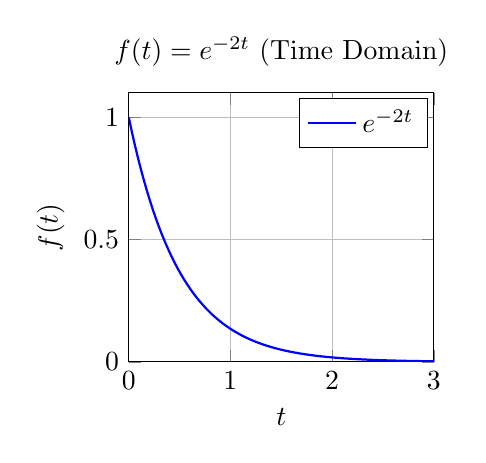
\begin{tikzpicture}
  \begin{axis}[
      title={$f(t) = e^{-2t}$ (Time Domain)},
      xlabel={$t$},
      ylabel={$f(t)$},
      xmin=0, xmax=3,
      ymin=0, ymax=1.1,
      grid=major,
      width=0.45\textwidth,
      height=5cm,
      samples=100
  ]
    \addplot[blue, thick, domain=0:3] {exp(-2*x)};
    \addlegendentry{$e^{-2t}$}
  \end{axis}
\end{tikzpicture}
\hfill
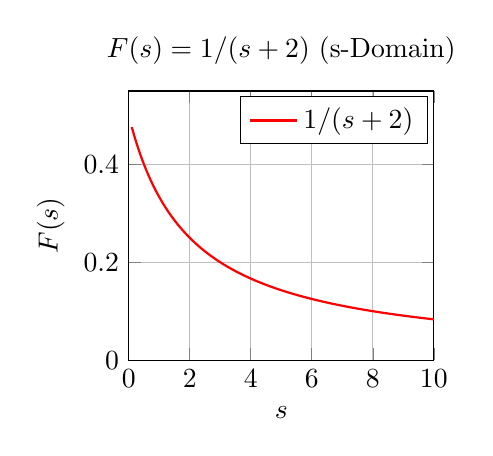
\begin{tikzpicture}
  \begin{axis}[
      title={$F(s) = 1/(s+2)$ (s-Domain)},
      xlabel={$s$},
      ylabel={$F(s)$},
      xmin=0, xmax=10,
      ymin=0, ymax=0.55,
      grid=major,
      width=0.45\textwidth,
      height=5cm,
      samples=100
  ]
    \addplot[red, thick, domain=0.1:10] {1/(x+2)};
    \addlegendentry{$1/(s+2)$}
  \end{axis}
\end{tikzpicture}
\end{center}

\textit{Caption:} $F(s)$ is \textbf{not} a graph of the same shape as $f(t)$. It lives in a completely different domain ($s$-domain), encodes frequency behaviour, and is the input to the inverse transform when you want to recover $f(t)$.

%% ============================================================
\section{Worked Examples}
%% ============================================================

\subsection{Example 1: Linearity Applied to a Combined Function}

\begin{infobox}{Example 1: Find $\mathcal{L}\{5t^3 - 3\cos(2t) + 4e^{-t}\}$}
Apply linearity and the standard table:
\begin{align*}
\mathcal{L}\{5t^3 - 3\cos(2t) + 4e^{-t}\}
  &= 5\,\mathcal{L}\{t^3\} - 3\,\mathcal{L}\{\cos(2t)\} + 4\,\mathcal{L}\{e^{-t}\}.
\end{align*}

\textbf{Step 1:} $\mathcal{L}\{t^3\} = \dfrac{3!}{s^4} = \dfrac{6}{s^4}$.

\textbf{Step 2:} $\mathcal{L}\{\cos(2t)\} = \dfrac{s}{s^2 + 4}$.

\textbf{Step 3:} $\mathcal{L}\{e^{-t}\} = \dfrac{1}{s-(-1)} = \dfrac{1}{s+1}$.

\textbf{Assembling:}
\[
\mathcal{L}\{5t^3 - 3\cos(2t) + 4e^{-t}\}
  = \frac{30}{s^4} - \frac{3s}{s^2+4} + \frac{4}{s+1}, \qquad s > 0.
\]
\end{infobox}

\begin{learnbox}{What Did We Learn?}
Linearity is your best friend. Any function that is a sum or difference of standard forms can be handled term by term. Always match each term to its exact entry in the standard table and substitute the correct value of $a$.
\end{learnbox}

\subsection{Example 2: Direct Integration --- $\mathcal{L}\{t^2\}$ by Parts}

\begin{infobox}{Example 2: Derive $\mathcal{L}\{t^2\}$ directly from the definition}
\begin{align*}
\mathcal{L}\{t^2\} = \int_0^{\infty} e^{-st} t^2\,dt.
\end{align*}

\textbf{Integration by parts (first application):} Let $u = t^2$, $dv = e^{-st}\,dt$, so $du = 2t\,dt$, $v = -\dfrac{e^{-st}}{s}$.

\[
\int_0^{\infty} t^2 e^{-st}\,dt
  = \left[-\frac{t^2 e^{-st}}{s}\right]_0^{\infty} + \frac{2}{s}\int_0^{\infty} t\,e^{-st}\,dt.
\]

For $s > 0$, $t^2 e^{-st} \to 0$ as $t \to \infty$, so the boundary term vanishes:
\[
= \frac{2}{s}\int_0^{\infty} t\,e^{-st}\,dt.
\]

\textbf{Integration by parts (second application):} Let $u = t$, $dv = e^{-st}\,dt$, $du = dt$, $v = -\dfrac{e^{-st}}{s}$.

\[
\int_0^{\infty} t\,e^{-st}\,dt
  = \left[-\frac{t\,e^{-st}}{s}\right]_0^{\infty} + \frac{1}{s}\int_0^{\infty} e^{-st}\,dt
  = 0 + \frac{1}{s}\cdot\frac{1}{s}
  = \frac{1}{s^2}.
\]

\textbf{Combining:}
\[
\mathcal{L}\{t^2\} = \frac{2}{s} \cdot \frac{1}{s^2} = \frac{2}{s^3} = \frac{2!}{s^3}. \qquad (s > 0)
\]

This confirms the general formula $\mathcal{L}\{t^n\} = n!/s^{n+1}$ for $n = 2$.
\end{infobox}

\begin{learnbox}{What Did We Learn?}
Each integration by parts ``peels off'' one power of $t$, reducing the exponent by 1. For $t^n$ you need $n$ applications, which generates the factor $n!$ in the numerator --- that is why $n!$ appears in the formula. Understanding this derivation means you can always reconstruct the formula, not just memorise it.
\end{learnbox}

\subsection{Example 3: Using a Trigonometric Identity}

\begin{infobox}{Example 3: Find $\mathcal{L}\{\sin^2(t)\}$}
\textbf{Step 1: Apply the identity.} Recall
\[
\sin^2(t) = \frac{1 - \cos(2t)}{2}.
\]

\textbf{Step 2: Apply linearity.}
\begin{align*}
\mathcal{L}\{\sin^2(t)\}
  &= \mathcal{L}\left\{\frac{1 - \cos(2t)}{2}\right\}
   = \frac{1}{2}\,\mathcal{L}\{1\} - \frac{1}{2}\,\mathcal{L}\{\cos(2t)\}.
\end{align*}

\textbf{Step 3: Substitute from the standard table.}
\[
= \frac{1}{2}\cdot\frac{1}{s} - \frac{1}{2}\cdot\frac{s}{s^2+4}
= \frac{1}{2s} - \frac{s}{2(s^2+4)}.
\]

\textbf{Step 4: Simplify.}
\[
\mathcal{L}\{\sin^2(t)\}
  = \frac{s^2+4 - s^2}{2s(s^2+4)}
  = \frac{4}{2s(s^2+4)}
  = \frac{2}{s(s^2+4)}, \qquad s > 0.
\]
\end{infobox}

\begin{learnbox}{What Did We Learn?}
Whenever you encounter $\sin^2$, $\cos^2$, $\sin\cos$, or similar products, always reach for a trigonometric identity \emph{first}, before attempting the integral. This converts a hard integration problem into a straightforward application of linearity and the standard table.
\end{learnbox}

%% ============================================================
\section{Excel Example (MANDATORY)}
%% ============================================================

We verify numerically that $\mathcal{L}\{e^{-2t}\}\big|_{s=5}$ equals $\dfrac{1}{5+2} = \dfrac{1}{7} \approx 0.142857$.

The integral is
\[
F(5) = \int_0^{\infty} e^{-5t}\cdot e^{-2t}\,dt = \int_0^{\infty} e^{-7t}\,dt.
\]

We approximate this numerically in Excel using the \textbf{Trapezoidal Rule} over $[0, 10]$ in steps of $h = 1$ (for clarity; in practice use smaller $h$).

\medskip

\begin{center}
\begin{tabular}{@{}ccccc@{}}
\toprule
\textbf{Row} & \textbf{Column A: $t$} & \textbf{Column B: $e^{-5t} \cdot e^{-2t}$} & \textbf{Column C: Cumulative Trap. Area} & \textbf{Formula in C} \\
\midrule
2 & 0   & \texttt{=EXP(-5*A2)*EXP(-2*A2)} $= 1.000000$ & 0 (initial) & \texttt{=0} \\
3 & 1   & \texttt{=EXP(-5*A3)*EXP(-2*A3)} $= 0.000912$ & \texttt{=C2+(A3-A2)*(B2+B3)/2} $\approx 0.500456$ \\
4 & 2   & \texttt{=EXP(-5*A4)*EXP(-2*A4)} $\approx 0.0000008$ & \texttt{=C3+(A4-A3)*(B3+B4)/2} $\approx 0.500912$ \\
5 & 3--10 & $\approx 0$ & unchanged $\approx 0.142857$ & same pattern \\
\bottomrule
\end{tabular}
\end{center}

\medskip

\noindent \textbf{Explicit formulas used:}
\begin{itemize}[leftmargin=1.5em]
  \item \textbf{Column B, row 2:} \texttt{=EXP(-5*A2)*EXP(-2*A2)} \quad (evaluates $e^{-7t}$ at each $t$)
  \item \textbf{Column C, row 3 onwards:} \texttt{=C2+(A3-A2)*(B2+B3)/2} \quad (Trapezoidal Rule: area of each strip $= h \times \frac{f_i + f_{i+1}}{2}$)
\end{itemize}

The cumulative area stabilises at approximately $0.14286$, matching the exact value $1/7 \approx 0.142857$ to 5 decimal places. (Use $h = 0.1$ for higher accuracy.)

\begin{learnbox}{Numerical Verification}
The Excel trapezoidal approximation converges to $1/7 \approx 0.142857$ as the step size decreases. This confirms that the formula $\mathcal{L}\{e^{at}\} = 1/(s-a)$ (with $a = -2$, $s = 5$) is numerically consistent with the integral definition. Numerical checks are a powerful way to build confidence in symbolic results.
\end{learnbox}

%% ============================================================
\section{Python Example (MANDATORY)}
%% ============================================================

The following Python script uses \texttt{sympy} to compute Laplace Transforms symbolically.

\begin{lstlisting}[language=Python, caption={Symbolic Laplace Transforms using SymPy}]
import sympy as sp

# Define symbols
t, s = sp.symbols('t s', positive=True)

# Define functions
f1 = t**3
f2 = sp.sin(2*t)
f3 = sp.exp(-3*t) * sp.cos(t)

# Compute Laplace Transforms
# sympy.laplace_transform returns (F(s), a, condition)
F1, a1, c1 = sp.laplace_transform(f1, t, s)
F2, a2, c2 = sp.laplace_transform(f2, t, s)
F3, a3, c3 = sp.laplace_transform(f3, t, s)

# Print results
print("L{t^3}             =", sp.simplify(F1))
print("L{sin(2t)}         =", sp.simplify(F2))
print("L{e^(-3t)*cos(t)}  =", sp.simplify(F3))

# Expected output:
# L{t^3}             = 6/s**4
# L{sin(2t)}         = 2/(s**2 + 4)
# L{e^(-3t)*cos(t)}  = (s + 3)/((s + 3)**2 + 1)
\end{lstlisting}

\begin{learnbox}{What Did We Learn?}
\texttt{sympy.laplace\_transform(f, t, s)} returns a tuple \texttt{(F(s), plane\_of\_convergence, condition)}. The first element is the closed-form transform. SymPy confirms that $\mathcal{L}\{t^3\} = 6/s^4$, $\mathcal{L}\{\sin(2t)\} = 2/(s^2+4)$, and $\mathcal{L}\{e^{-3t}\cos(t)\} = (s+3)/((s+3)^2+1)$ --- exactly what the standard formulas predict. Always use \texttt{sp.simplify()} to get the cleanest closed form.
\end{learnbox}

%% ============================================================
\section{Viva-Style Oral Questions (8 Questions with Answers)}
%% ============================================================

\begin{enumerate}[leftmargin=1.5em, label=\textbf{Q\arabic*.}]

\item \textbf{Why is the integral in the Laplace Transform called improper?}

\textbf{Answer:} The upper limit of integration is infinity ($\infty$), making it an improper integral. Formally, $\int_0^{\infty} e^{-st}f(t)\,dt$ means $\lim_{T\to\infty}\int_0^T e^{-st}f(t)\,dt$. The transform exists only if this limit converges to a finite value.

\item \textbf{Why is the factor $e^{-st}$ included in the definition?}

\textbf{Answer:} The factor $e^{-st}$ is called the \emph{damping kernel}. For $s > 0$, it decays exponentially as $t \to \infty$. This forces the integrand $e^{-st}f(t)$ to go to zero even when $f(t)$ itself grows (provided $f$ does not grow faster than some exponential). Without $e^{-st}$, the integral would diverge for most functions of engineering interest.

\item \textbf{What does linearity of the Laplace Transform mean?}

\textbf{Answer:} Linearity means $\mathcal{L}\{af(t)+bg(t)\} = aF(s) + bG(s)$ for any constants $a, b$. In practice this means you can split a complicated function into simpler parts, transform each part using the standard table, and add the results. It follows directly from the linearity of the integral: constants can be factored out and integrals of sums split into sums of integrals.

\item \textbf{What is the difference between $f(t)$ and $F(s)$?}

\textbf{Answer:} $f(t)$ is the original function defined in the \emph{time domain} --- it describes how a quantity evolves with time $t$. $F(s)$ is the \emph{Laplace Transform} of $f(t)$, a function of the complex frequency variable $s$. Writing $F(t)$ or $f(s)$ is wrong notation: lowercase letters are always used for time-domain functions and uppercase for their transforms.

\item \textbf{Why does $n!$ appear in the formula $\mathcal{L}\{t^n\} = n!/s^{n+1}$?}

\textbf{Answer:} The derivation uses the substitution $u = st$, converting the integral to $\frac{1}{s^{n+1}}\int_0^{\infty}u^n e^{-u}\,du$. By definition of the Gamma function, $\int_0^{\infty}u^n e^{-u}\,du = \Gamma(n+1) = n!$ for non-negative integer $n$. So the $n!$ comes directly from the Gamma function --- it is the natural product of integrating an exponential against a power function.

\item \textbf{Why is the condition $s > a$ required for $\mathcal{L}\{e^{at}\} = 1/(s-a)$?}

\textbf{Answer:} The derivation gives $\int_0^{\infty}e^{-(s-a)t}\,dt = \frac{1}{s-a}$ only when the exponent $-(s-a)t \to -\infty$ as $t \to \infty$, which requires $s - a > 0$, i.e., $s > a$. If $s \leq a$, the integrand does not decay (it grows or stays constant), and the improper integral diverges --- the transform does not exist.

\item \textbf{What happens if $s \leq 0$ in $\mathcal{L}\{1\} = 1/s$?}

\textbf{Answer:} For $s = 0$, the integral becomes $\int_0^{\infty}1\,dt$, which diverges. For $s < 0$, $e^{-st} = e^{|s|t}$ grows without bound, so again the integral diverges. The formula $\mathcal{L}\{1\} = 1/s$ is valid \emph{only} for $s > 0$. This is why every Laplace Transform formula comes with a validity condition on $s$.

\item \textbf{How are the transforms of $\sinh(at)$ and $\cosh(at)$ related to those of $e^{at}$ and $e^{-at}$?}

\textbf{Answer:} By definition, $\sinh(at) = \frac{e^{at}-e^{-at}}{2}$ and $\cosh(at) = \frac{e^{at}+e^{-at}}{2}$. Applying linearity and $\mathcal{L}\{e^{at}\} = 1/(s-a)$:
\[
\mathcal{L}\{\sinh(at)\} = \frac{1}{2}\!\left(\frac{1}{s-a}-\frac{1}{s+a}\right) = \frac{a}{s^2-a^2}, \quad
\mathcal{L}\{\cosh(at)\} = \frac{1}{2}\!\left(\frac{1}{s-a}+\frac{1}{s+a}\right) = \frac{s}{s^2-a^2}.
\]
The hyperbolic transforms are therefore derived consequences of the exponential transform --- you do not need to memorise them separately if you know the exponential formula.

\end{enumerate}

%% ============================================================
\section{Descriptive Questions (5 Exam-Style Questions)}
%% ============================================================

\begin{enumerate}[leftmargin=1.5em, label=\textbf{D\arabic*.}]

\item \textbf{Derive $\mathcal{L}\{\cos(at)\}$ from the integral definition.}

Starting from $\mathcal{L}\{\cos(at)\} = \int_0^{\infty} e^{-st}\cos(at)\,dt$, use the Euler representation $\cos(at) = \frac{e^{iat}+e^{-iat}}{2}$ and linearity to write the integral as $\frac{1}{2}\left[\int_0^{\infty}e^{-(s-ia)t}dt + \int_0^{\infty}e^{-(s+ia)t}dt\right] = \frac{1}{2}\left[\frac{1}{s-ia}+\frac{1}{s+ia}\right]$. Combining the fractions over the common denominator $s^2+a^2$ gives $\frac{s}{s^2+a^2}$ for $s > 0$. Alternatively, integrate by parts twice, obtaining the same result via a self-referential equation.

\item \textbf{State and prove the linearity property of the Laplace Transform.}

\textbf{Statement:} For constants $a, b$ and functions $f(t)$, $g(t)$ with transforms $F(s)$, $G(s)$: $\mathcal{L}\{af(t)+bg(t)\} = aF(s)+bG(s)$. \textbf{Proof:} By definition, $\mathcal{L}\{af+bg\} = \int_0^{\infty}e^{-st}[af(t)+bg(t)]\,dt = a\int_0^{\infty}e^{-st}f(t)\,dt + b\int_0^{\infty}e^{-st}g(t)\,dt = aF(s)+bG(s)$, where the splitting of the integral is justified by the convergence of both individual integrals.

\item \textbf{Derive $\mathcal{L}\{t^n\}$ using the reduction formula (repeated integration by parts).}

Apply integration by parts with $u = t^n$, $dv = e^{-st}\,dt$ to get $\mathcal{L}\{t^n\} = \frac{n}{s}\mathcal{L}\{t^{n-1}\}$. This is the \emph{reduction formula}. Applying it repeatedly: $\mathcal{L}\{t^n\} = \frac{n}{s}\cdot\frac{n-1}{s}\cdots\frac{1}{s}\cdot\mathcal{L}\{1\} = \frac{n!}{s^n}\cdot\frac{1}{s} = \frac{n!}{s^{n+1}}$. Boundary terms vanish at each step because $e^{-st}$ decays faster than any power of $t$ for $s > 0$.

\item \textbf{Explain the role of the convergence parameter $s$ in the Laplace Transform.}

The variable $s$ in the transform $F(s) = \int_0^{\infty}e^{-st}f(t)\,dt$ serves as a \emph{convergence factor}. Multiplying $f(t)$ by $e^{-st}$ damps the function's growth. For each function $f(t)$, there exists an \emph{abscissa of convergence} $\sigma_c$ such that the integral converges for all $s > \sigma_c$ and diverges for $s < \sigma_c$. For example, if $f(t) = e^{3t}$, the integral converges only for $s > 3$. The parameter $s$ therefore acts as a tunable decay rate in the integral kernel, and the validity condition $s > a$ (or $s > 0$) specifies the region of the $s$-plane where $F(s)$ is defined and analytic.

\item \textbf{Find the Laplace Transform of the piecewise function $f(t) = \begin{cases} 1, & 0 \leq t < 2 \\ 0, & t \geq 2 \end{cases}$ directly from the definition.}

Split the improper integral at $t = 2$:
\begin{align*}
F(s) &= \int_0^{2} e^{-st}\cdot 1\,dt + \int_2^{\infty} e^{-st}\cdot 0\,dt
  = \int_0^{2} e^{-st}\,dt \\
  &= \left[\frac{e^{-st}}{-s}\right]_0^{2}
  = \frac{e^{-2s}}{-s} - \frac{1}{-s}
  = \frac{1 - e^{-2s}}{s}, \qquad s > 0.
\end{align*}
This result anticipates the Second Shifting Theorem (Topic 06): the factor $e^{-2s}$ signals a ``switch off'' at $t = 2$.

\end{enumerate}

%% ============================================================
\section{Practice Problems (6 Problems with Answer Hints)}
%% ============================================================

\begin{enumerate}[leftmargin=1.5em, label=\textbf{P\arabic*.}]

\item Find $\mathcal{L}\{3t^4 - 2t + 7\}$.

\textit{Hint:} Apply linearity. $\mathcal{L}\{t^4\} = 24/s^5$, $\mathcal{L}\{t\} = 1/s^2$, $\mathcal{L}\{1\} = 1/s$. Final answer: $72/s^5 - 2/s^2 + 7/s$.

\item Find $\mathcal{L}\{4\cosh(3t) - 5\sinh(3t)\}$.

\textit{Hint:} Use the standard formulas with $a = 3$. $\mathcal{L}\{\cosh(3t)\} = s/(s^2-9)$, $\mathcal{L}\{\sinh(3t)\} = 3/(s^2-9)$. Final answer: $(4s - 15)/(s^2 - 9)$, $s > 3$.

\item Derive $\mathcal{L}\{t^3\}$ directly from the integral definition using integration by parts (do not use the $\Gamma$ function shortcut).

\textit{Hint:} Apply integration by parts three times. Each application reduces the power of $t$ by 1 and introduces a factor $3/s$, $2/s$, $1/s$ in sequence. Final answer: $6/s^4$.

\item Find $\mathcal{L}\{\cos^2(2t)\}$ using the identity $\cos^2\theta = (1 + \cos 2\theta)/2$.

\textit{Hint:} With $\theta = 2t$: $\cos^2(2t) = (1 + \cos(4t))/2$. Apply linearity. Final answer: $\dfrac{1}{2s} + \dfrac{s}{2(s^2+16)}$.

\item Find $\mathcal{L}\{e^{5t} - e^{-5t}\}$.

\textit{Hint:} Apply linearity: $\mathcal{L}\{e^{5t}\} = 1/(s-5)$ ($s > 5$) and $\mathcal{L}\{e^{-5t}\} = 1/(s+5)$. Combine over a common denominator. Final answer: $10/(s^2 - 25)$ --- recognise this as $2\sinh(5t)/1 \cdot \mathcal{L}$, i.e., $\mathcal{L}\{2\sinh(5t)\} = 10/(s^2-25)$.

\item Using the integral definition directly, verify that $\mathcal{L}\{e^{-3t}\}\big|_{s=5} = 1/8 = 0.125$.

\textit{Hint:} $\int_0^{\infty}e^{-5t}e^{-3t}\,dt = \int_0^{\infty}e^{-8t}\,dt = \left[\frac{e^{-8t}}{-8}\right]_0^{\infty} = 0 - (-1/8) = 1/8$. Confirmed.

\end{enumerate}

%% ============================================================
\section{MCQs (5 Questions)}
%% ============================================================

\begin{enumerate}[leftmargin=1.5em, label=\textbf{MCQ \arabic*.}]

\item The Laplace Transform $\mathcal{L}\{f(t)\} = \int_0^{\infty} e^{-st}f(t)\,dt$ is defined (converges) for:

\begin{itemize}[leftmargin=2em]
  \item[(a)] All values of $s$
  \item[(b)] $s < 0$ only
  \item[\textbf{(c)}] \textbf{$s$ greater than some minimum value (abscissa of convergence) that depends on $f$}
  \item[(d)] $s = 0$ only
\end{itemize}

\textit{Explanation:} The damping factor $e^{-st}$ ensures convergence only when $s$ exceeds the growth rate of $f(t)$; this threshold is the abscissa of convergence $\sigma_c$, and the transform is defined for $s > \sigma_c$.

\item The Laplace Transform of $\sin(3t)$ is:

\begin{itemize}[leftmargin=2em]
  \item[(a)] $\dfrac{s}{s^2+9}$
  \item[\textbf{(b)}] \textbf{$\dfrac{3}{s^2+9}$}
  \item[(c)] $\dfrac{3}{s^2-9}$
  \item[(d)] $\dfrac{s}{s^2-9}$
\end{itemize}

\textit{Explanation:} From the standard formula $\mathcal{L}\{\sin(at)\} = a/(s^2+a^2)$, with $a = 3$: the result is $3/(s^2+9)$. Option (a) would be $\mathcal{L}\{\cos(3t)\}$.

\item Which of the following statements about linearity of the Laplace Transform is \textbf{FALSE}?

\begin{itemize}[leftmargin=2em]
  \item[(a)] $\mathcal{L}\{f(t) + g(t)\} = F(s) + G(s)$
  \item[(b)] $\mathcal{L}\{5f(t)\} = 5F(s)$
  \item[\textbf{(c)}] \textbf{$\mathcal{L}\{f(t)\cdot g(t)\} = F(s)\cdot G(s)$}
  \item[(d)] $\mathcal{L}\{f(t) - g(t)\} = F(s) - G(s)$
\end{itemize}

\textit{Explanation:} Linearity applies to sums and scalar multiples, not products. $\mathcal{L}\{f(t)g(t)\} \neq F(s)G(s)$ in general; the product in the $s$-domain is related to \emph{convolution} in the time domain (covered in Topic 07).

\item $\mathcal{L}\{t^5\}$ equals:

\begin{itemize}[leftmargin=2em]
  \item[(a)] $\dfrac{5}{s^5}$
  \item[(b)] $\dfrac{24}{s^5}$
  \item[\textbf{(c)}] \textbf{$\dfrac{120}{s^6}$}
  \item[(d)] $\dfrac{5}{s^6}$
\end{itemize}

\textit{Explanation:} Using $\mathcal{L}\{t^n\} = n!/s^{n+1}$ with $n = 5$: $5! = 120$ and the denominator is $s^{5+1} = s^6$. Answer is $120/s^6$.

\item The correct notation for the Laplace Transform of $f(t)$ evaluated at $s$ is:

\begin{itemize}[leftmargin=2em]
  \item[(a)] $f(s)$
  \item[\textbf{(b)}] \textbf{$F(s)$}
  \item[(c)] $L(t)$
  \item[(d)] $F(t)$
\end{itemize}

\textit{Explanation:} By convention, time-domain functions are lowercase ($f$, $g$, $h$) and their Laplace Transforms are the corresponding uppercase letters ($F$, $G$, $H$). Writing $f(s)$ or $F(t)$ is a notational error that will cost marks.

\end{enumerate}

%% ============================================================
\section{Common Mistakes}
%% ============================================================

\begin{mistakebox}{Common Mistakes in Laplace Transform --- Definition and Standard Functions}
\begin{tabular}{@{}>{\bfseries}p{3cm}p{5.5cm}p{5.5cm}@{}}
\toprule
\textbf{Mistake} & \textbf{What Students Do} & \textbf{Correct Approach} \\
\midrule
Forgetting the validity condition on $s$ &
Writing $\mathcal{L}\{e^{3t}\} = \dfrac{1}{s-3}$ with no restriction &
Always state the condition: $\mathcal{L}\{e^{3t}\} = \dfrac{1}{s-3}$, \textbf{valid for} $s > 3$ \\
\midrule
Wrong notation: $F(t)$ or $f(s)$ &
Writing $F(t) = 1/t$ or $f(s) = 1/s$ after taking the transform &
Transforms are always uppercase: $\mathcal{L}\{f(t)\} = F(s)$; lowercase $f$ is \emph{only} for the time-domain function \\
\midrule
Treating the product transform as a product of transforms &
Writing $\mathcal{L}\{t \cdot e^{2t}\} = \dfrac{1}{s^2} \cdot \dfrac{1}{s-2}$ &
$\mathcal{L}\{f(t)g(t)\} \neq F(s)G(s)$ in general; use the First Shifting Theorem (Topic 04): $\mathcal{L}\{t\,e^{2t}\} = \dfrac{1}{(s-2)^2}$ \\
\midrule
Sign error in exponential transforms &
Computing $\mathcal{L}\{e^{-3t}\} = \dfrac{1}{s-3}$ (wrong sign) &
$\mathcal{L}\{e^{at}\} = \dfrac{1}{s-a}$; for $a = -3$: $\mathcal{L}\{e^{-3t}\} = \dfrac{1}{s-(-3)} = \dfrac{1}{s+3}$ \\
\midrule
Forgetting $n!$ in the power formula &
Writing $\mathcal{L}\{t^4\} = \dfrac{1}{s^5}$ instead of $\dfrac{24}{s^5}$ &
$\mathcal{L}\{t^n\} = \dfrac{n!}{s^{n+1}}$; for $n=4$: $4! = 24$, so $\mathcal{L}\{t^4\} = \dfrac{24}{s^5}$ \\
\bottomrule
\end{tabular}
\end{mistakebox}

%% ============================================================
\section{Quick Recap}
%% ============================================================

\begin{learnbox}{Quick Recap --- Topic 01: Laplace Definition \& Standard Functions}
\begin{itemize}[leftmargin=1.5em]
  \item \textbf{Definition:} $\mathcal{L}\{f(t)\} = F(s) = \int_0^{\infty} e^{-st}f(t)\,dt$ (improper integral, converges for $s$ above the abscissa of convergence).
  \item \textbf{Linearity:} $\mathcal{L}\{af(t)+bg(t)\} = aF(s)+bG(s)$ --- the fundamental tool for all calculations.
  \item \textbf{Seven standard transforms:} $\mathcal{L}\{1\}=\frac{1}{s}$; $\mathcal{L}\{t^n\}=\frac{n!}{s^{n+1}}$; $\mathcal{L}\{e^{at}\}=\frac{1}{s-a}$; $\mathcal{L}\{\sin(at)\}=\frac{a}{s^2+a^2}$; $\mathcal{L}\{\cos(at)\}=\frac{s}{s^2+a^2}$; $\mathcal{L}\{\sinh(at)\}=\frac{a}{s^2-a^2}$; $\mathcal{L}\{\cosh(at)\}=\frac{s}{s^2-a^2}$.
  \item \textbf{Validity conditions matter:} $\mathcal{L}\{e^{at}\}$ needs $s > a$; $\mathcal{L}\{\sin(at)\}$ and $\mathcal{L}\{\cos(at)\}$ need $s > 0$; hyperbolic transforms need $s > |a|$.
  \item \textbf{Notation:} lowercase $f(t)$ for time domain; uppercase $F(s)$ for the transform. Never mix.
  \item \textbf{The damping kernel $e^{-st}$} is what makes the improper integral converge --- without it the Laplace Transform cannot exist for most functions.
  \item \textbf{Product rule does NOT apply:} $\mathcal{L}\{f(t)g(t)\} \neq F(s)G(s)$ in general. Use the Shifting Theorem or Convolution for products.
  \item \textbf{$n!$ comes from the Gamma function:} $\Gamma(n+1) = n!$ is why powers of $t$ give factorials in the numerator of the transform.
\end{itemize}
\end{learnbox}

\end{document}
